%!TEX root = ../main.tex

\chapter{Background biologico}\label{chp:biological-background}

La cellula è l'unità fondamentale della vita. La cellula è una piccola miscela acquosa con componenti chimici, racchiusi in una membrana, e possiede l'eccezionale capacità di replicarsi. Il primo elemento che permette di distinguere le cellule è la presenza di un nucleo. Vengono definite \textsl{procarioti} le cellule senza nucleo — che sono le più diffuse e compongono organismi unicellulari come i batteri e gli archei — mentre sono chiamate \textsl{eucarioti} le cellule che contengono un nucleo — le quali sono in genere più grandi e più complesse e costituiscono forme di vita multicellulari come animali, piante e funghi\,\cite{alberts2015essential}.

All'interno della cellula eucariote (Figura\,\ref{fig:cell}), immersi nel \textsl{citoplasma}, sono presenti diversi \textsl{organuli}, i quali svolgono una particolare funzione ciascuno. I \textsl{mitocondri} sono gli organuli più diffusi.
% 
\begin{figure}[b!]
    \centering
    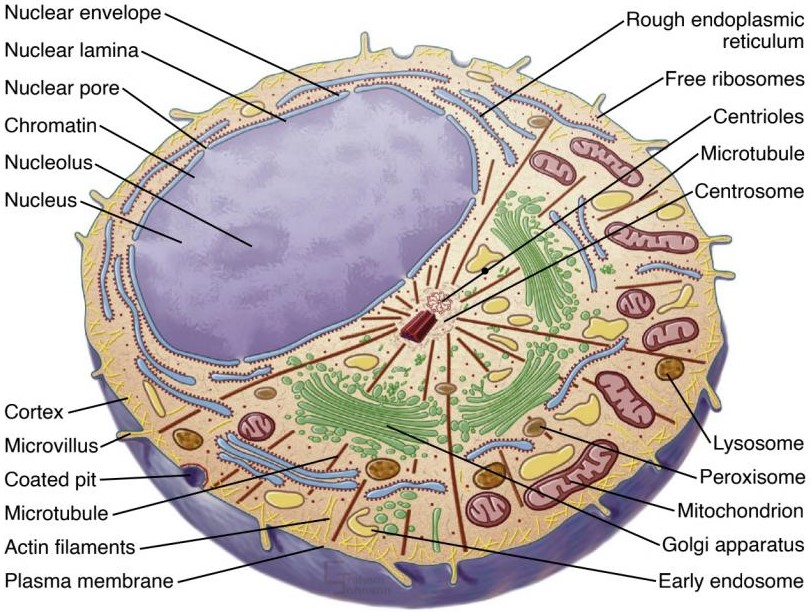
\includegraphics[width=.65\textwidth]{assets/cell.jpg}
    \caption[Rappresentazione schematica della cellula eucariote.]{Rappresentazione schematica della cellula eucariote; si possono notare i principali organuli tra cui i mitocondri, lisosomi e perossiomi, il reticolo endoplasmatico, e il nucleo\,\cite{pollard2022cell}.}\label{fig:cell}
\end{figure}
% 
Il loro compito è quello di generare energia chimica per la cellula: attraverso il processo di ossidazione di zuccheri e grassi, viene creata una sostanza che viene utilizzata nella maggior parte delle attività cellulari\footnote{Questa sostanza è detta \textsl{adenosintrifosfato} o ATP ed ha una struttura simile ad un nucleotide: è infatti composta dall'Adenina, da uno zucchero e da tre gruppi fosfati.}; questo processo è anche chiamato \textsl{respirazione cellulare} perché consumando l'ossigeno viene rilasciata anidride carbonica. Oltre ad essere la fonte energetica primaria della cellula, i mitocondri hanno anche importanti ruoli nella regolazione del metabolismo, del ciclo cellulare, delle risposte antivirali e anche della morte della cellula\,\cite{alberts2015essential, chinnery2003mitochondria, mcbride2006mitochondria}.

Il \textsl{reticolo endoplasmatico} è invece un organulo molto esteso e svolge molteplici funzioni. Tra questi compiti rientrano quelli di traslocazione di proteine e il ripiegamento delle proteine (\textsl{protein folding})\,\cite{alberts2015essential, voeltz2002structural}. I \textsl{lisosomi} si occupano di degradare e riciclare gli scarti cellulari e giocano un ruolo fondamentale per l'omeostasi della cellula\footnote{Con omeostasi cellulare si intende l'insieme di meccanismi necessari per mantenere ad un livello ottimale le funzioni della cellula.}, il suo sviluppo e il suo invecchiamento\,\cite{ballabio2016awesome, yang2021lysosome, dell2000lysosome}. Infine, i \textsl{perossiomi} sono delle piccole vescicole che forniscono un ambiente protetto per gestire molecole tossiche come gli acidi grassi i quali sono smaltiti tramite la $\beta$-ossidazione\,\cite{alberts2015essential, islinger2012peroxisome}.

L'organulo più importante della cellula rimane il \textsl{nucleo}. Racchiuso nell'\textsl{involucro nucleare}, all'interno di questo organulo sono presenti tutte le informazioni genetiche, racchiuse in una lunga molecola di acido desossiribonucleico (comunemente noto come DNA), che, una volta impacchettato forma il \textsl{cromosoma}\,\cite{pollard2022cell, alberts2015essential}. La molecola di DNA è una struttura a doppia elica formata da \textsl{nucleotidi}. Osservando la Figura\,\ref{fig:dna}, i nucleotidi sono composti a loro volta da tre elementi fondamentali: una \textsl{base azotata}, uno \textsl{zucchero} e un \textsl{gruppo fosfato}\footnote{I gruppi fosfati hanno una carica negativa e forniscono alla molecola le proprietà di un acido.}.
% 
\begin{figure}[b!]
    \centering
    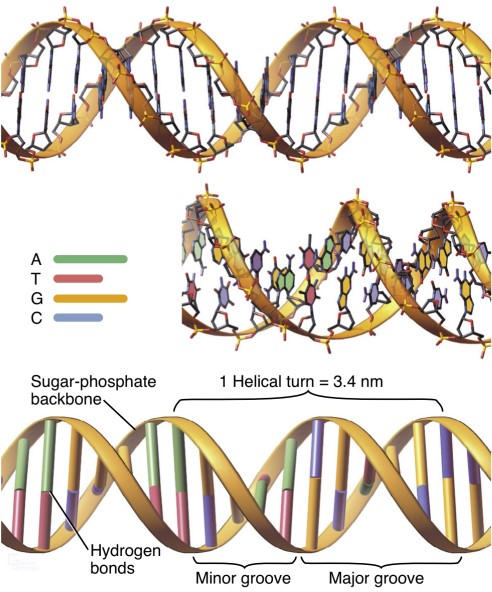
\includegraphics[width=\textwidth]{assets/dna.jpg}
    \caption[Rappresentazione schematica del DNA.]{Rappresentazione schematica del DNA in cui si possono osservare le coppie di basi azotate, legate tra loro attraverso gli zuccheri e i gruppi fosfati\,\cite{nhgri_dna_image}.}\label{fig:dna}
\end{figure}
% 
Le basi azotate sono quattro — Adenina (A), Citosina (C), Guanina (G) e Timina (T) — e si uniscono tra loro mediante dei legami ad idrogeno e secondo un preciso criterio: l'Adenina si lega solamente con la Timina (formando il legame \textit{AT}) mentre la Citosina si unisce solo con la Guanina (creando la coppia \textit{CG})\,\cite{fonseca2000hydrogen, sahu2011identification}. Si osserva infine che il nucleotide di una coppia e quello successivo si legano mediante zucchero e gruppo fosfato sempre allo stesso modo: il gruppo fosfato di un nucleotide si lega sempre allo zucchero dell'altro. Di conseguenza, preso un filamento della doppia elica, le due estremità non sono uguali in quanto una termina con un gruppo fosfato (terminazione $5^\prime$) e l'altra con uno zucchero (terminazione $3^\prime$).

Attraverso una serie di ripiegamenti, una molecola di DNA lunga circa due metri riesce a raggomitolarsi in un cromosoma di grandezza inferiore a 2 micron (Figura\,\ref{fig:dna-packaging}). Il processo di \textit{DNA-packaging} inizia avvolgendo la doppia elica di DNA attorno a delle proteine dette \textsl{istoni} e formando dei \textsl{nucleosomi}. In secondo luogo i nucleosomi si ammassano vicini tra loro formando una fibra, chiamata \textsl{cromatina} che, a sua volta si impacchetta su se stessa creando il cromosoma\,\cite{jansen2011nucleosome, zheng2010packaging}.

\begin{figure}[b!]
    \centering
    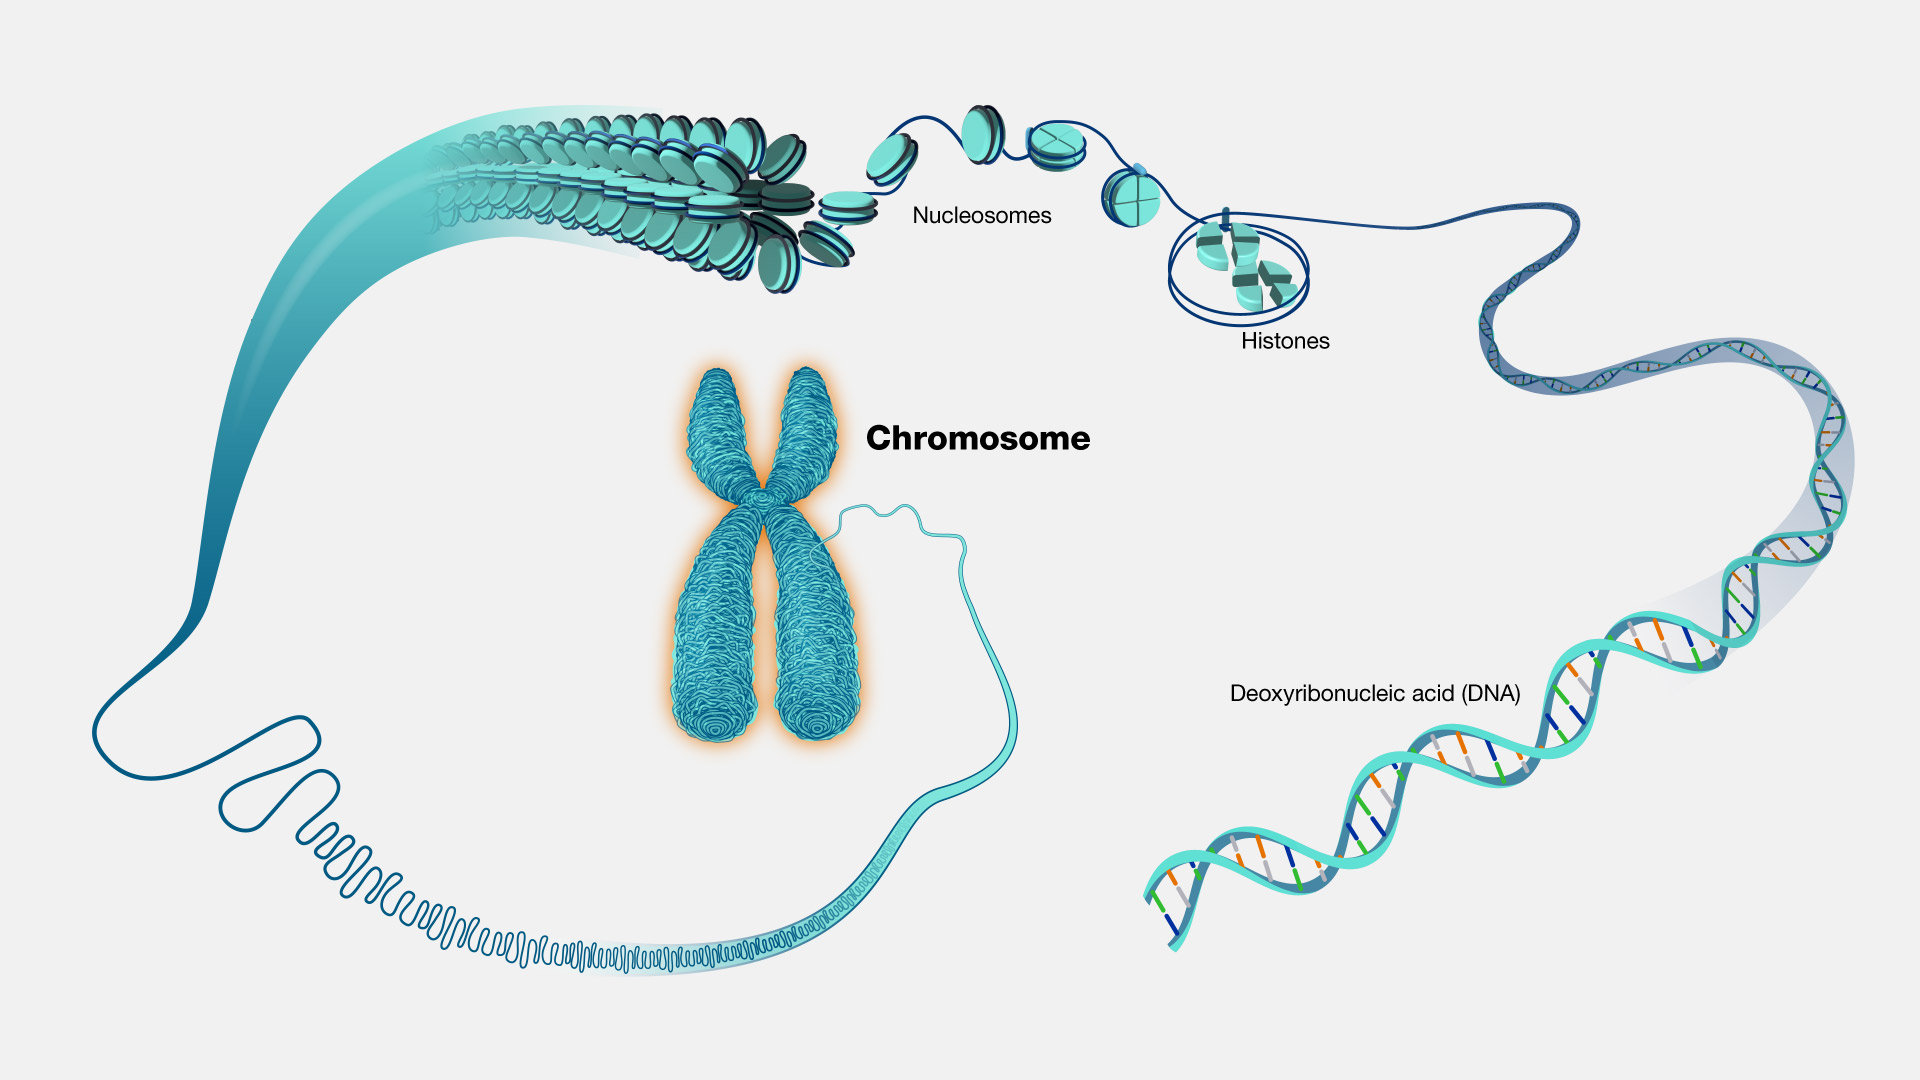
\includegraphics[width=\textwidth]{assets/dna-packaging.jpg}
    \caption[Il processo di impacchettamento del DNA.]{Il processo di impacchettamento del DNA che permette di compattare la struttura a doppia eilca nel cromosoma\,\cite{nhgri_chromosome_image}.}\label{fig:dna-packaging}
\end{figure}

\section{Dogma centrale}

La rilevanza del DNA è data delle informazioni essenziali che questa molecola contiene. Tali informazioni risiedono nei geni, che sono delle sequenze genomiche che codificano uno o più prodotti biologici operativi\,\cite{gerstein2007gene}. L'\textsl{espressione genica} è il processo che permette di utilizzare i dati contenuti nel gene per la creazione di macromolecole, come le proteine. Per esempio, le cellule della pelle a contatto con luce solare intensa possono esprimere geni che regolano la pigmentazione della pelle\,\cite{white2009gene}. L'espressione genica è divisa in due fasi principali: la \textsl{trascrizione} — che si occupa di produrre delle molecole di RNA che rispecchino il gene da esprimere — e la \textsl{traduzione} — la quale traduce le informazioni dell'RNA sintetizzando la proteina.

Nella prima fase dell'espressione genica, è necessario trascrivere il DNA in una molecola molto simile ovvero l'RNA — chiamato anche acido ribonucleico. Questa molecola differisce dall'acido desossiribonucleico per una base azotata — anziché la Timina è presente l'Uracile (U) — e per lo zucchero — da desossiribosio a ribosio\,\cite{alberts2002dna}. La trascrizione del DNA in RNA inizia quando delle proteine, chiamate \textsl{fattori di trascrizione}, attratte dagli \textit{enhancer} del DNA, riconoscono la regione che delimita l'inizio della molecola del gene da esprimere, detta \textsl{zona promotrice}. Dopo aver riconosciuto l'inizio della sequenza, queste proteine permettono ad un enzima chiamato \textsl{RNA polimerasi} di attaccarsi ed aprire la doppia elica del DNA\,\cite{cramer2019organization}. Una volta aperta la doppia elica, inizia la vera e propria trascrizione in RNA:\@ il filamento del DNA viene preso come modello per la creazione dell'RNA;\@ in particolare il nucleotide dell'RNA sarà il complementare rispetto a quello del DNA (di conseguenza $A\rightarrow U$, $C\rightarrow G$, $G\rightarrow C$ e $T\rightarrow A$). Così facendo l'acido ribonucleico viene creato un nucleotide alla volta, analizzando quello del DNA\,\cite{alberts2002dna}. La trascrizione termina nel momento in cui gli enzimi e le proteine incontrano la regione terminatrice del gene che determina la separazione dal filamento e la terminazione dell'RNA \textsl{messaggero} (\textsl{mRNA}) che contiene le informazioni presenti nel gene da esprimere. L'intero processo di trascrizione è illustrato nella Figura\,\ref{fig:dna-transcription}.

\begin{figure}[b!]
    \centering
    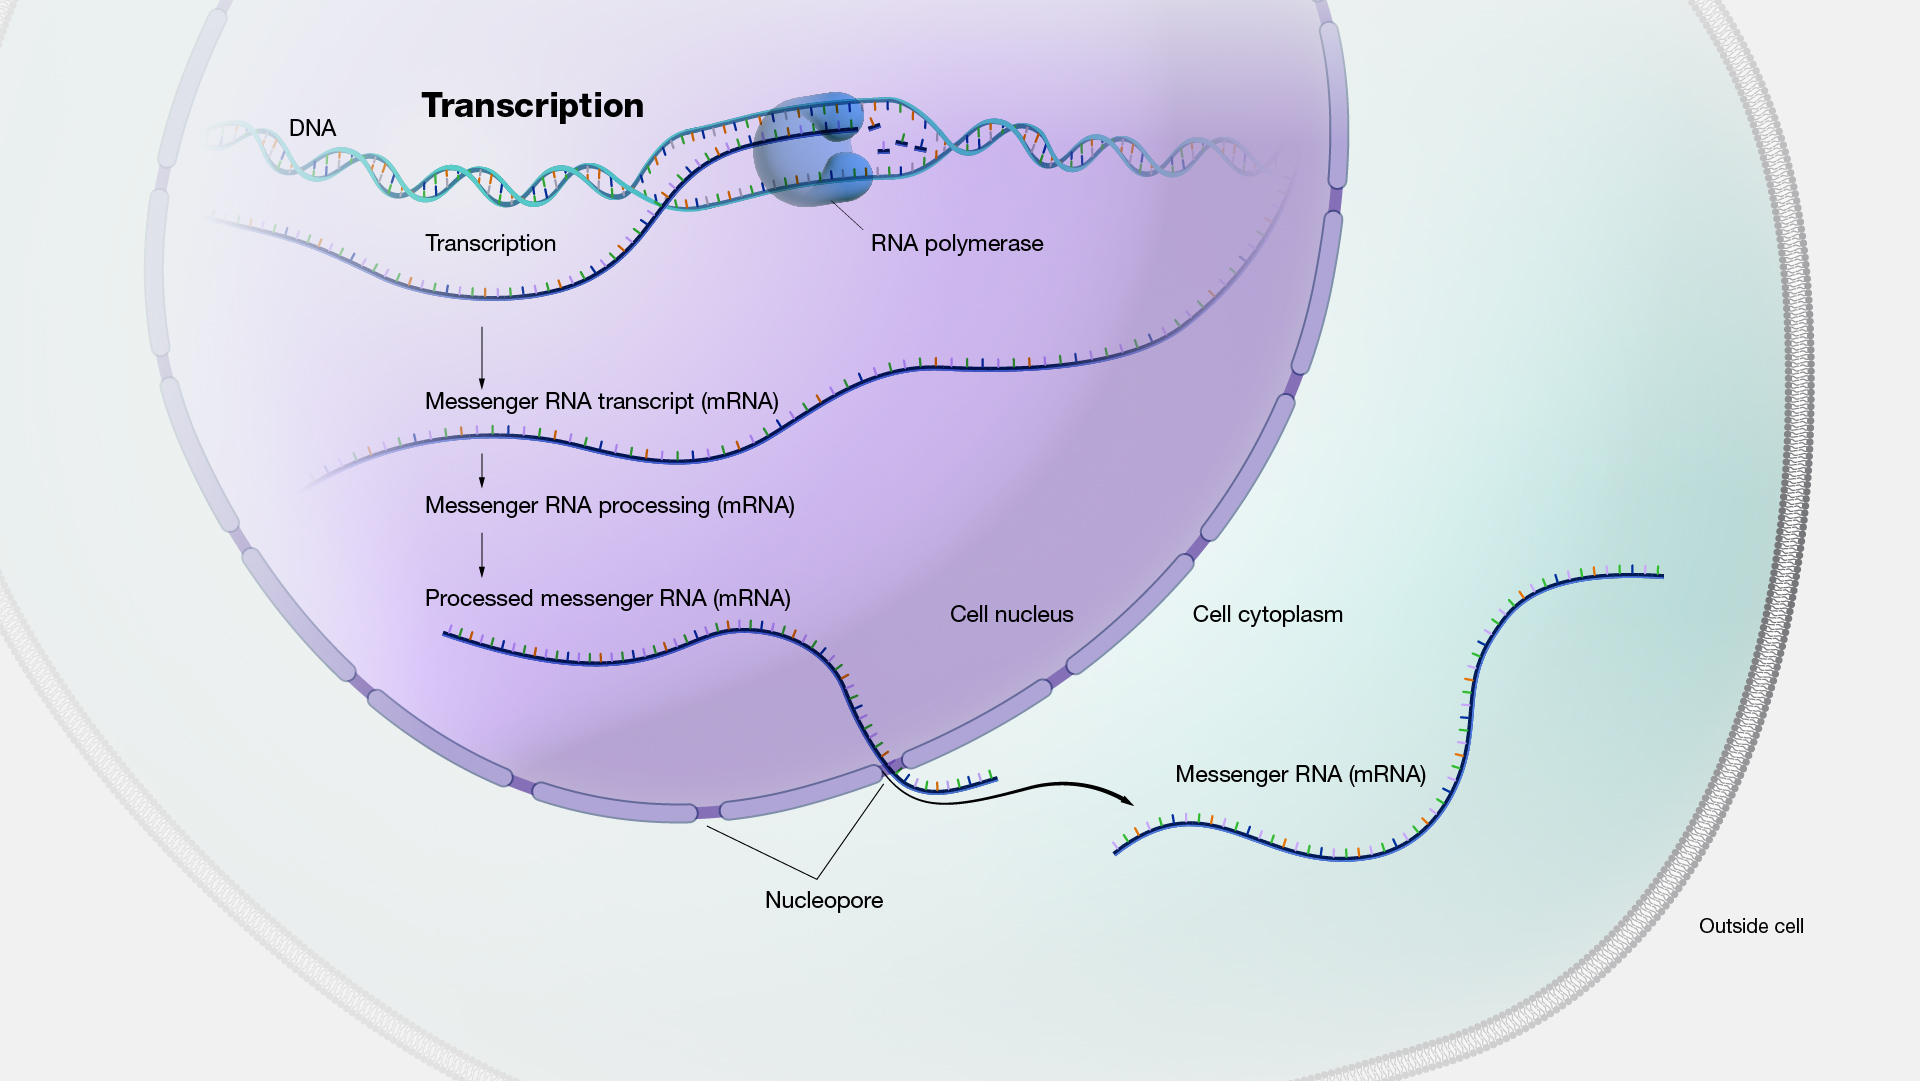
\includegraphics[width=\textwidth]{assets/dna-transcription.jpg}
    \caption[Il processo di trascrizione del DNA in RNA.]{Il processo di trascrizione del DNA del gene in RNA mediante la RNA polimerasi\,\cite{nhgri_transcription_image}.}\label{fig:dna-transcription}
\end{figure}

Prima di uscire dal nucleo l'RNA messaggero subisce una serie di elaborazioni necessarie per rendere le informazioni immagazzinare sicure: diverse sono le malattie che emergono per mutazioni presenti nell'mRNA tra cui la distrofia miotonica\footnote{Le distrofie miotoniche sono patologie che colpiscono principalmente l'apparato muscolo-scheletrico.}\,\cite{philips2000rna}. La prima elaborazione viene chiamata $5^\prime$-\textit{end capping} e si occupa di aggiungere alla terminazione $5^\prime$ dell'mRNA una Guanina attraverso un collegamento inusuale che garantisce maggiore stabilità alla molecola. In secondo luogo avviene lo \textit{splicing} che si occupa di rimuovere le zone non codificanti — dette \textsl{introni}— dal gene trascritto mantenendo solo quelle che verranno utilizzate per essere sintetizzate in proteine — gli \textsl{esoni} — e quindi facilitando il processo di traduzione. Infine con il $3^\prime$-\textit{end processing} viene aggiunta alla terminazione $3^\prime$ dell'mRNA una coda di Adenine — datta anche \textit{poly}A \textit{tail} — che, in maniera molto simile al $5^\prime$-\textit{end capping} garantisce una stabilità del filamento di acido ribonucleico\,\cite{hocine2010rna, livingstone2010mechanisms}.

Dopo essere uscito dal nucleo attraverso i \textsl{pori}, l'RNA messaggero raggiunge il citoplasma ed è pronto per iniziare la seconda fase dell'espressione genica, la traduzione. La traduzione non è altro che la traduzione dell'mRNA in un \textsl{polipeptide}, ovvero una sequenza di aminoacidi che compongono la proteina. Gli aminoacidi sono più di 20, di conseguenza anziché codificare un solo nucleotide dell'RNA messaggero, vengono codificati tre nucleotidi alla volta: questa tripletta viene chiamata \textsl{codone}. Durante la fase della traduzione, giocano un ruolo fondamentale i \textsl{ribosomi} i quali sono degli organuli nei quali avviene la traduzione. I ribosomi sono composti da due sotto unità, ciascuna delle quali ha tre siti per l'RNA di \textsl{trasporto} (\textsl{tRNA}). Delle due sotto unità del ribosoma, quella dimensionalmente minore si lega all'mRNA e agli \textsl{anticodoni} (sequenze specifiche di tre basi nel tRNA) e controlla che la traduzione avvenga con successo. La sotto unità più voluminosa invece si prende carico di catalizzare il legame peptidico tra l'aminoacido trasportato dal tRNA e la catena di aminoacidi in crescita\,\cite{ramakrishnan2002ribosome, lemonniermarathon, livingstone2010mechanisms}. In questo modo i ribosomi, analizzando codone dopo codone riescono a creare la catena polipeptidica mediante l'RNA di trasporto, come mostrato nella Figura\,\ref{fig:mrna-translation}.

\begin{figure}[b!]
    \centering
    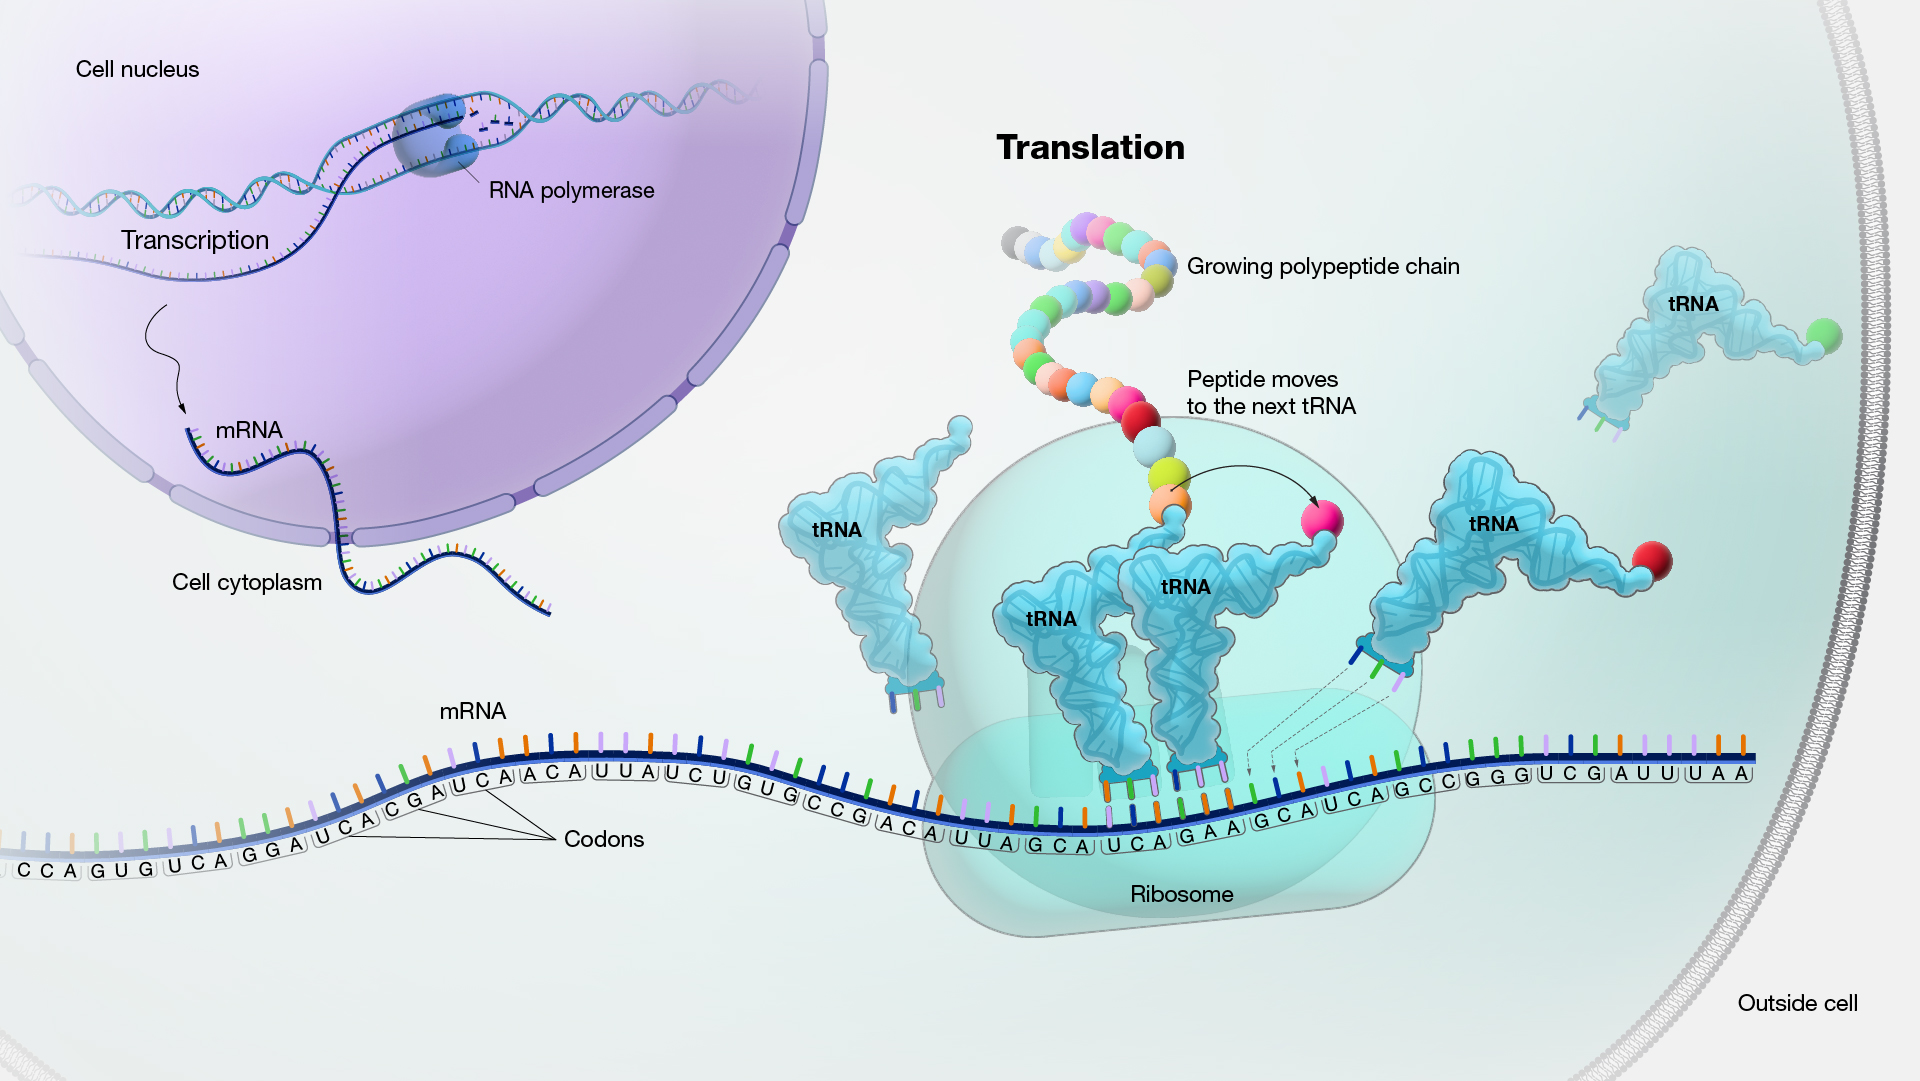
\includegraphics[width=\textwidth]{assets/mrna-translation.jpg}
    \caption[Il processo di traduzione da mRNA a polipeptide.]{Il processo di traduzione da RNA messaggero a polipeptide attraverso il tRNA e i ribosomi\,\cite{nhgri_translation_image}.}\label{fig:mrna-translation}
\end{figure}

Una volta creata la sequenza polipeptidica, inizia il processo di ripiegamento della proteina. In maniera molto simile a quanto visto per l'impacchettamento del DNA nel cromosoma, la sequenza di polipeptidi inizialmente si arrotola creando delle bobine che sono comunemente chiamate $\alpha$\textit{-helix}. Queste ultime poi si ripiegano nuovamente arrivando alla struttura terziaria della proteina, ovvero la proteina tridimensionale effettiva\,\cite{schulz2013principles}. Una volta creata la proteina il gene è stato espresso definitivamente. Questo passaggio di informazioni dal DNA alla creazione della proteina è gergo definito come il \textsl{dogma della biologia molecolare}.

Come accennato all'inizio del capitolo, la cellula possiede la notevole capacità di replicarsi. In genere una cellula si duplica durante la crescita e lo sviluppo dell'organismo, quando deve essere rimpiazzata o rigenerata oppure nella riproduzione asessuata di alcuni micro organismi\,\cite{bavle2014mitosis}. Il processo replicazione cellulare, chiamato \textsl{mitosi}, è preceduto dall'\textsl{interfase}, processo fondamentale in cui la cellula cresce di dimensioni e il DNA nei cromosomi si duplica, favorendo la replicazione cellulare. La mitosi può essere suddivisa in quattro fasi principali\,\cite{walczak2010mechanisms, bavle2014mitosis, li2020theoretical, sullivan2007finishing} le quali sono riassunte anche nella Figura\,\ref{fig:mitosis}:
\begin{enumerate}
    \item Nella \textsl{profase} i cromosomi duplicati si condensano nel nucleo ed iniziano ad avvicinarsi dei microtuboli al nucleo, chiamati \textsl{centrosomi}; allo stesso tempo la membrana nucleare inizia a svanire;
    \item Dopo che i microtuboli si sono attaccati ai cromosomi (fase intermedia detta \textsl{prometafase}) si giunge alla \textsl{metafase}, situazione in cui tutti i cromosomi sono allineati lungo la linea equatoriale della cellula;
    \item Durante l'\textsl{anafase}, ciascuna coppia di cromosomi si divide e raggiunge i poli della cellula;
    \item La fase finale della mitosi è la \textsl{telofase} nella quale le due cellule si dividono; le membrane nucleari delle due cellule si riformano attorno ai cromosomi divisi.
\end{enumerate}

\begin{figure}[b!]
    \centering
    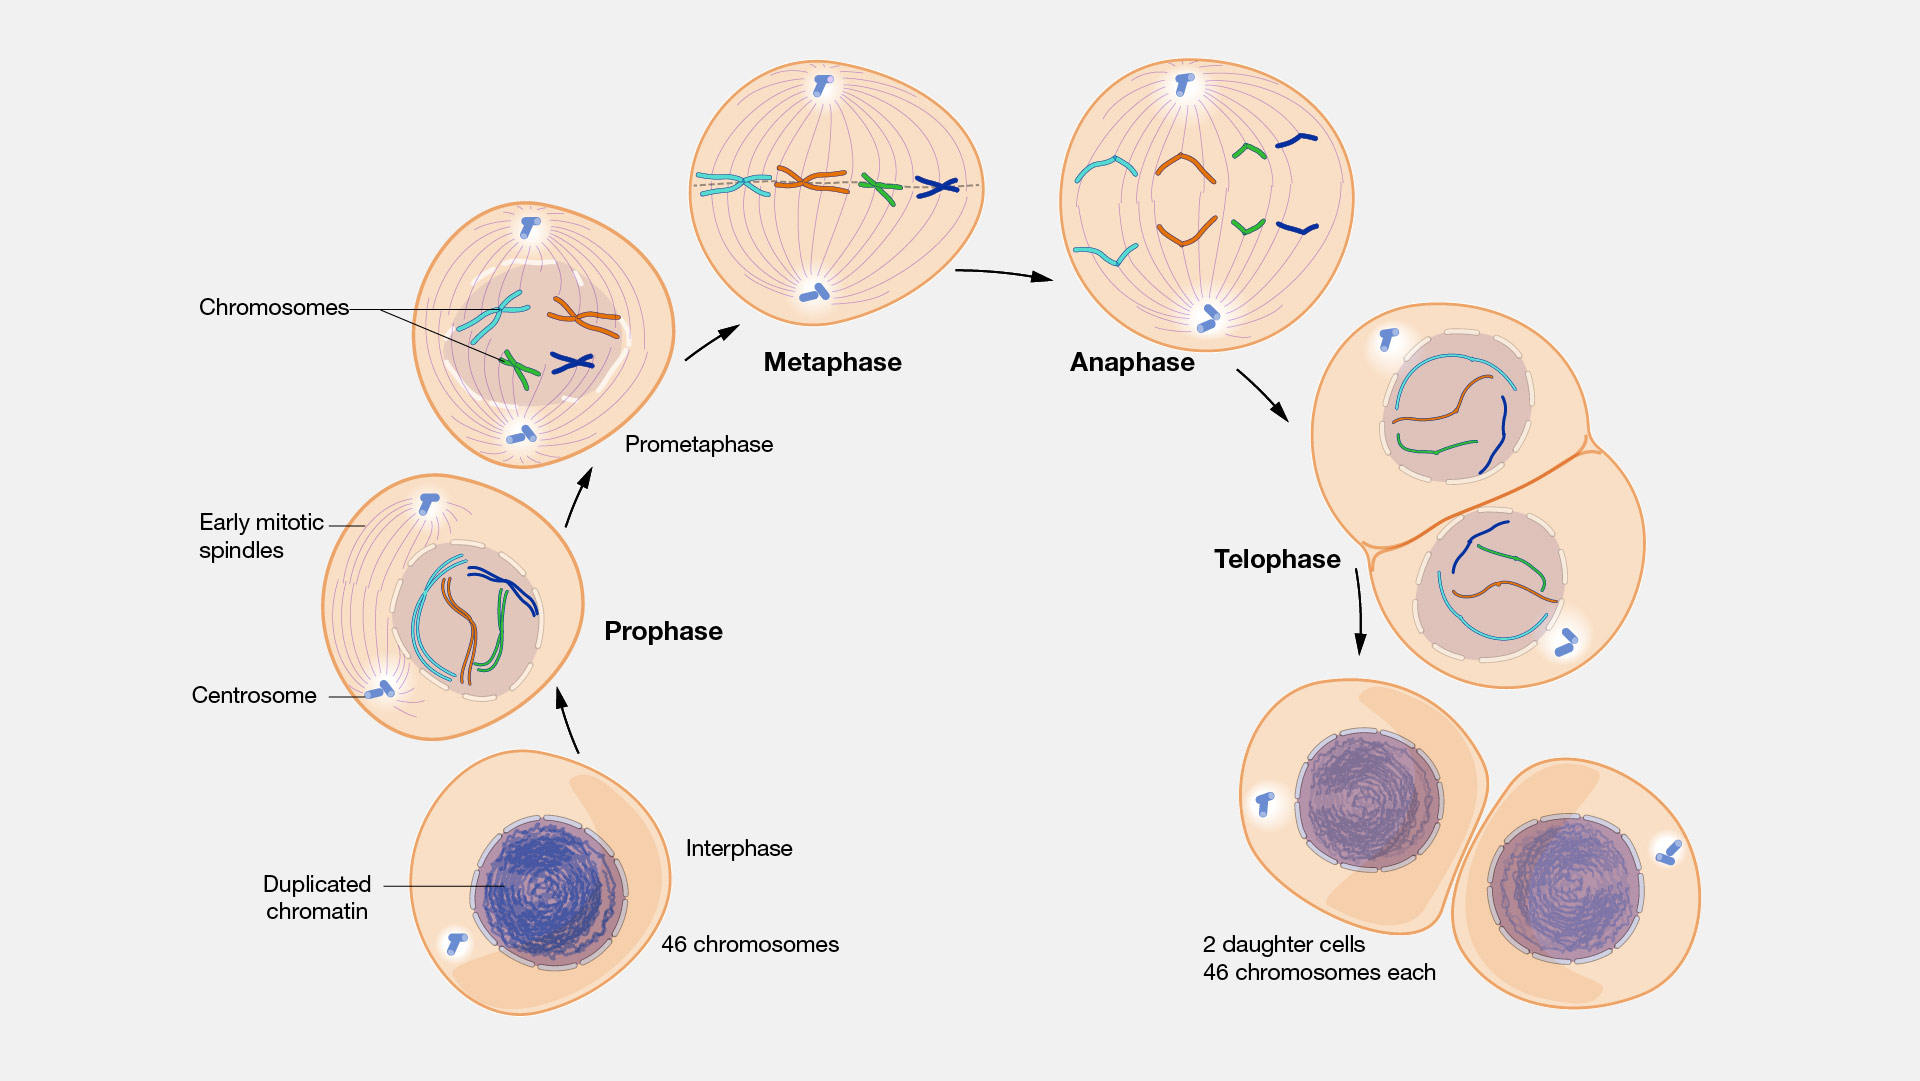
\includegraphics[width=\textwidth]{assets/mitosis.jpg}
    \caption[La mitosi cellulare.]{Rappresentazione delle quattro fasi che comprendono la mitosi cellulare\,\cite{nhgri_mitosis_image}.}\label{fig:mitosis}
\end{figure}

Affinché la mitosi abbia successo, è prima necessario duplicare il DNA all'interno della cellula. Il processo di replicazione di DNA che precede la mitosi è anche definito come \textsl{fase di sintesi} — \textit{S-phase}. La duplicazione del DNA inizia con l'identificazione dell'\textsl{origine della replicazione}, ovvero una sequenza del DNA che specifica da quale punto della sequenza il DNA deve essere replicato (ci sono più di cento mila siti che segnalano un punto di orine nel DNA di una cellula). Una \textsl{proteina iniziatrice} è legata al punto di origine promuovendo l'attaccamento al DNA del \textsl{replisoma} che è composto da un enzima chiamato \textsl{elicasi} che si occupa di dividere i due filamenti di DNA procedendo nella direzione $5^\prime \to 3^\prime$.\@ A questo punto il \textsl{RNA prime} inizia la sintesi del DNA favorendo l'attaccamento della \textsl{DNA polimerasi} entrambi i filamenti per duplicare il DNA.\@ Essendo che il genoma è complementare, un filamento avrà un verso $5^\prime \to 3^\prime$ (\textit{leading strand}) mentre l'altro filamento avrà verso opposto, $3^\prime \to 5^\prime$ (\textit{lagging strand}). Di conseguenza, nel filamento concorde al replisoma, la polimerasi non incontrerà problemi nella duplicazione, invece nel filamento $3^\prime \to 5^\prime$ il DNA dovrà essere duplicato a segmenti, detti \textsl{frammenti di Okazaki} che verranno collegati tramite la \textsl{DNA ligasi}\,\cite{laskey1989s, bell2002dna, dutta1997initiation, 2017727}. La Figura\,\ref{fig:dna-replication} racchiude quanto descritto sulla fase di sintesi.

\begin{figure}[b!]
    \centering
    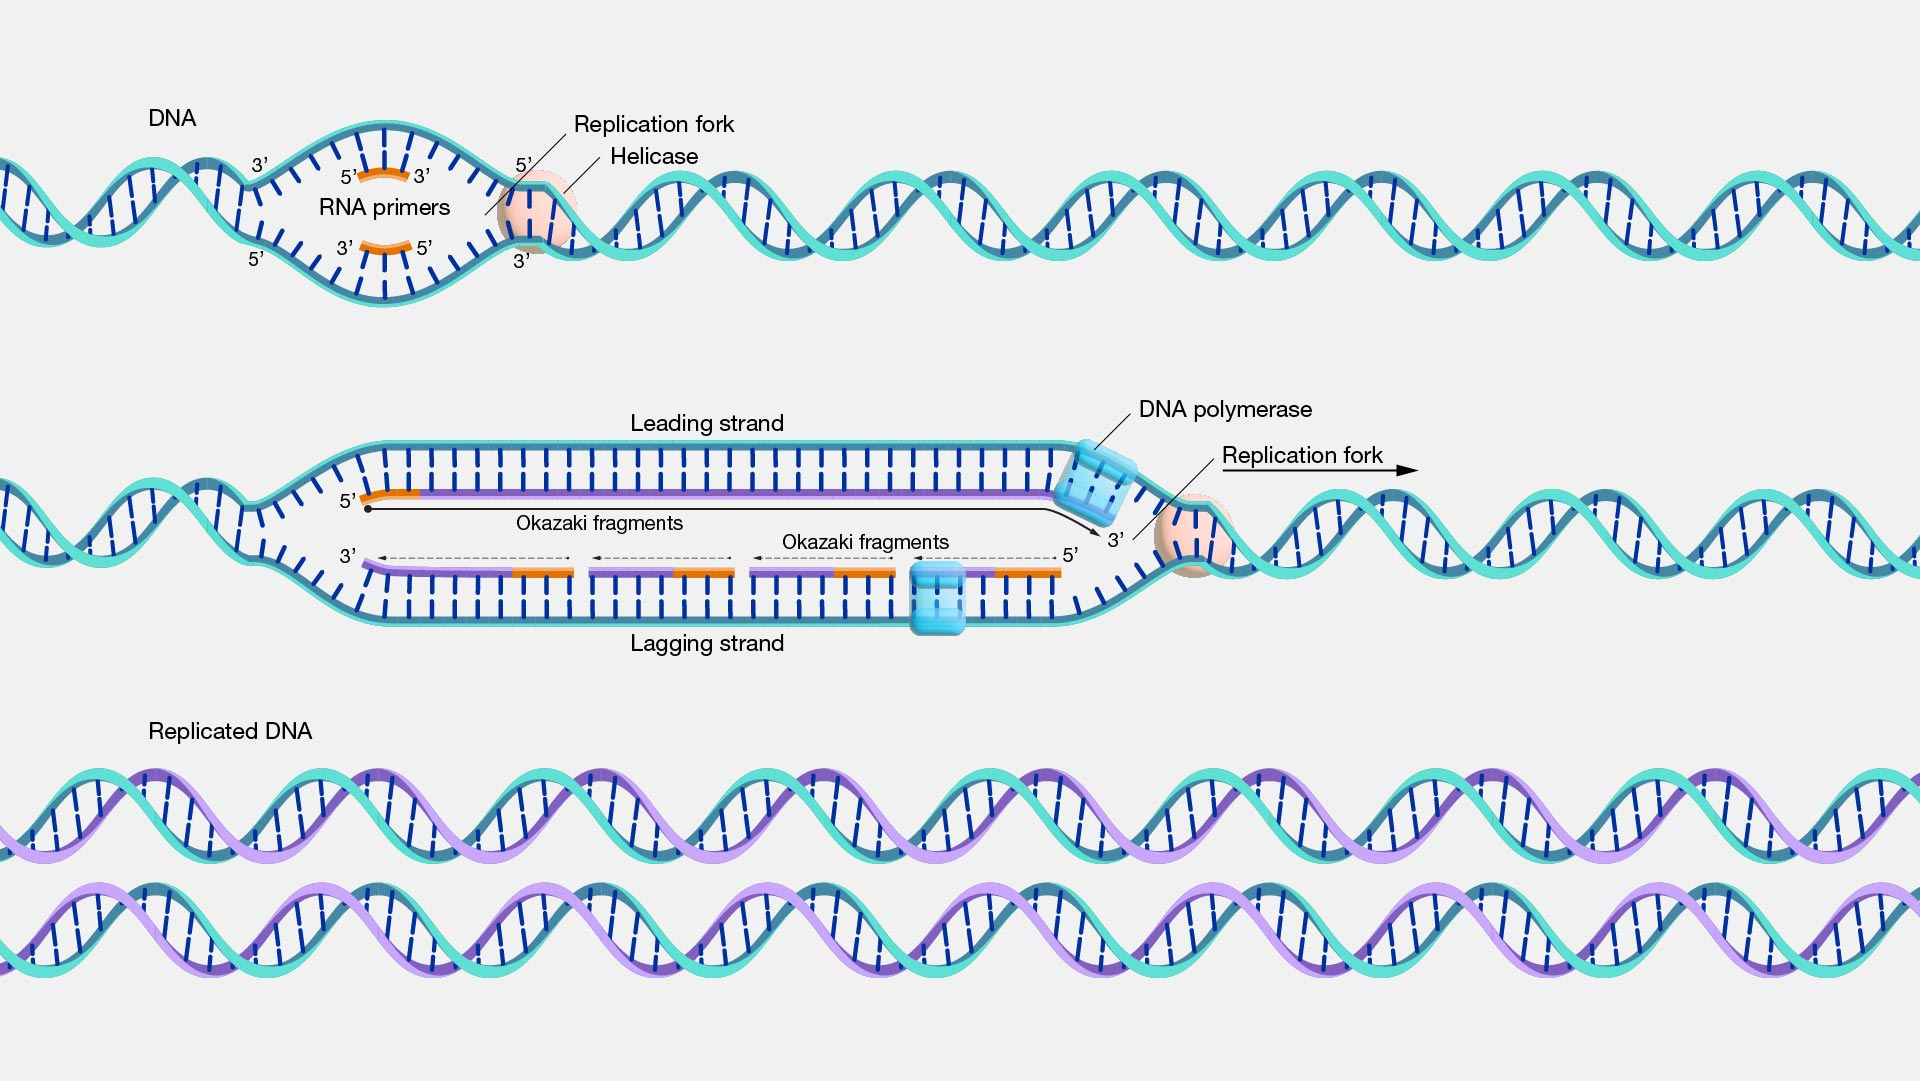
\includegraphics[width=\textwidth]{assets/dna-replication.jpg}
    \caption[Il processo di replicazione del DNA.]{Il processo di replicazione del DNA durante la fase di sintesi\,\cite{nhgri_dna_replication_image}.}\label{fig:dna-replication}
\end{figure}

\section{Varianti non codificanti}

Come descritto fino ad ora, il ruolo del DNA è fondamentale in quanto trasmesso da cellula a cellula durante la replicazione per poi essere utilizzato nell'espressione genica creando le proteine. Alle regioni del DNA che prendono parte al processo di espressione di un gene, si contrappongono le regioni che non vengono codificate, come le zone intensificatrici e promotrici del DNA e gli introni dei geni. Anche se queste sequenze non vengono effettivamente espresse, ricoprono un ruolo fondamentale nell'espressione genica (Figura\,\ref{fig:dna-transcription} e Figura\,\ref{fig:mrna-translation}) e durante la duplicazione del DNA (Figura\,\ref{fig:dna-replication}). Proprio per questo motivo le mutazioni in queste zone possono indurre a disturbi genetici critici. Ciò nonostante non si è ancora in grado di comprendere a fondo gli effetti che queste particolari mutazioni hanno. Risulta quindi importante continuare a studiare le varianti non codificanti e gli effetti collaterali genetici che provocano.


\todo{spiega in maniera più approfondita la varianti non codificianti}